\documentclass{report}

%------------------------------------------------------------
% All packages are here defined
%------------------------------------------------------------
%\usepackage{mathtools}
\usepackage[table]{xcolor}
\usepackage[a4paper]{geometry}
\usepackage{vmargin}
\usepackage[english]{babel}
\usepackage[english]{varioref}
\usepackage[utf8]{inputenc}
\usepackage{graphicx}
\usepackage{array}
\usepackage{float}
\usepackage{tabularx}
\usepackage{hhline}
\usepackage{amsmath}
\usepackage{amssymb}
\usepackage{hyperref}
\usepackage{url}
\usepackage{fancyhdr}
\usepackage{setspace}
\usepackage{listings}
\usepackage{color}
\usepackage{abstract}
\usepackage{titlesec}
\usepackage{multirow}
\usepackage{datetime}
\usepackage{varwidth}
\usepackage{svg}
\usepackage{epsfig}
\usepackage{blindtext}
\usepackage{xcolor}

%----------------------------------------------------
%	MARGINS
%----------------------------------------------------
\setmarginsrb  { 1.5in}  % left margin
                        { 0.6in}  % top margin
                        { 1.0in}  % right margin
                        { 0.8in}  % bottom margin
                        {  20pt}  % head height
                        {0.25in}  % head sep
                        {   9pt}  % foot height
                        { 0.3in}  % foot sep
%----------------------------------------------------------------------------------------

%-------------------------------------------------
% Colors defination
%--------------------------------------------------
\definecolor{dkgreen}{rgb}{0,0.6,0}
\definecolor{gray}{rgb}{0.5,0.5,0.5}
\definecolor{mauve}{rgb}{0.58,0,0.82}
\definecolor{navyblue}{rgb}{0.0, 0.0, 0.5}



%-------------------------------------------------
% JAVA language settings for code insertion
%---------------------------------------------------
\lstset{frame=tb,
  language=Java,
  aboveskip=3mm,
  belowskip=3mm,
  showstringspaces=false,
  columns=flexible,
  basicstyle={\small\ttfamily},
  numbers=none,
  numberstyle=\tiny\color{gray},
  keywordstyle=\color{blue},
  commentstyle=\color{dkgreen},
  stringstyle=\color{mauve},
  breaklines=true,
  breakatwhitespace=true
  tabsize=3
}

%----------------------------------------------------------
% Horizontal line formation
%--------------------------------------------------------
\newcommand{\Hline}{\par
  \begin{center}
   \line(1,0){400}
   \end{center}
}


%------------------------------------------------------
% heading formation for chapters and other headings
%------------------------------------------------------
\titleformat
{\chapter} % command
[display] % shape
{\bfseries\LARGE} % format
{\Huge{Chapter.\ \thechapter}} % label
{0.5ex} % sep
{
\rule{\textwidth}{1pt}%
\vspace{1ex}
\centering
} % before-code
[
\vspace{-0.5ex}%
\rule{\textwidth}{0.3pt}
] % after-code

%-------------------------------------------------------
%heading formation for Acknowledgement
%-------------------------------------------------------


%---------------------------------------------------------
% Others
%----------------------------------------------------------

\newdateformat{mydate}{\monthname[\THEMONTH] \THEYEAR}	
%\geometry{a4paper}
\renewcommand{\abstractnamefont}{\normalfont\LARGE\bfseries}


%------------------------------------------------------
% Beginning main document
%---------------------------------------------------

\begin{document}
\pagenumbering{gobble} 


%----------------------------------------------------------------------------------------
%	Title page
%----------------------------------------------------------------------------------------
\begin{titlepage}
\begin{center}


{\huge \bfseries Graph Theoretical Algorithms For }\\[0.3cm]
{\huge \bfseries Structural Comparison Of Java Source}\\[0.3cm] % Thesis title
{\huge \bfseries  And Byte Code }\\[0.3cm]
\Hline

\begin{center}
\large{Submitted By}\\[0.2cm]
\textbf{\Large{Artem Garishin}}\\[2cm]
\end{center}


\includegraphics[width=0.50\textwidth]{Figures/FH_logo}\\[0.5cm]
\textbf{\large FB2: Faculty of Computer Science and Engineering}\\[1cm]


\large \textit{This thesis presented for the degree of\\ Master of Science} \\
\textit{in the}\\[0.2cm]
\textbf{\textcolor{navyblue}{High Integrity Systems}}\\[2.5cm] % Research group name and department name

\begin{center}


\begin{varwidth}{0.8\textwidth}
\raggedright
\textbf{Research Supervisor}: {Prof. Dr. Sergej Alekseev}\\[0.2cm] % Supervisor name - remove the \href bracket to remove the link  
\textbf{Co-Supervisor}: {Prof. Dr. Matthias Wagner}\\ % Supervisor name - remove the \href bracket to remove the link  
[3cm]
\end{varwidth}\\[3cm]
\end{center}



{\large \mydate\today}\\[1cm] % Date
%\includegraphics{Logo} % University/department logo - uncomment to place it

\vfill

\end{center}

\end{titlepage}


%----------------------------------------------------------
%Declaration
%---------------------------------------------------------
%\doublespacing%
\onehalfspacing
\null\vfil
%\vskip 60\p@
\begin{center}{\huge\bf Legal Declaration\par}\end{center}
%\vskip 60\p@
\null
I declare that this thesis document is completely my own work and all used references have been clearly cited. I have not submitted this assignment in the context of an examination to any other examination board or person.\\[2.5cm]

\begin{flushleft}
Signature:\\
\rule[1em]{25em}{0.5pt} % This prints a line for the signature
 
Location, Date:\\
\rule[1em]{25em}{0.5pt} % This prints a line to write the date
\end{flushleft}


%-----------------------------------------------------------------
% Abstract 
%----------------------------------------------------------
\newpage
\pagestyle{fancy}
\fancyhead{}
\renewcommand{\headrulewidth}{0pt}
\renewcommand{\footrulewidth}{0.4pt}
\pagenumbering{Roman}
%\doublespacing
\begin{abstract}
\large

TODO:
\par 
This should be a 1-page (maximum) summary of your work. What environment for development has been used, experimental results 
An abstract is a summary in your own words of the Thesis It is not evaluative and must not include your personal opinions. The purpose of an abstract is to give a reader sufficient information for him or her to decide whether it would be worthwhile reading the entire article or book. An abstract should aim at giving as much information as possible in as few words as possible. 
\par 
Goal of this work is to search out the most optimal ways to compare different pieces of code. So far there are two techniques for code comparison: a normal text comparison and visual compare. Normal text-compare can be not sufficient to analyse two pieces of code, or to find a similarity between them. For that reason a structural/graph compare opens a doors to discover more possibilities of comparison. 

\end{abstract}

%--------------------------------------------------------
%Acknowledgement
%-------------------------------------------------------
\newpage
%\null\vfil
%\vskip 60\p@
\begin{center}{\huge\bf Acknowledgments\par}\end{center}
%\vskip 60\p@
\null
I would like to take this time to thank Frankfurt University of Applied Sciences for all of the resources which they provided me in order to pursuing my master study in computer science and make this thesis possible.\vspace{5 mm}

\noindent I would like to express my sincere gratitude to Prof. Dr. Sergej Alekseev and Prof. Dr. Matthias Wagner for their patient guidance, encouragement and advice which they provided me throughout this thesis work.

%----------------------------------------------------------------------
% Some configurations
%-------------------------------------------------------

\newpage
\tableofcontents
\listoffigures
\listoftables

%--------------------------------------------------------
%Abbreviations
%-------------------------------------------------------
\newpage
\setstretch{1.5}
%\null\vfil
%\vskip 60\p@
\Hline
\begin{center}{\huge\bf Abbreviations\par}\end{center}
\Hline
%\vskip 60\p@
\vspace{10mm}
\null

\noindent
\textbf{TDMC} \hspace{20 mm} \textbf{T}op \textbf{D}own \textbf{M}ax \textbf{C}ommon \\
\textbf{BUMC} \hspace{20 mm} \textbf{B}ottom \textbf{U}p \textbf{M}ax \textbf{C}ommon \\
\textbf{BCV} \hspace{24 mm}  \textbf{B}yte \textbf{C}ode \textbf{V}isualizer \\
\textbf{SCV} \hspace{25 mm}  \textbf{S}ource \textbf{C}ode \textbf{V}isualizer \\
\textbf{CFGF} \hspace{22 mm} \textbf{C}ontrol \textbf{F}low \textbf{G}raph  \textbf{F}actory \\
\textbf{TC} \hspace{27 mm}   \textbf{T}ext \textbf{C}ompare \\
\textbf{MBM} \hspace{22 mm} \textbf{M}aximum \textbf{B}ipartite \textbf{M}atching \\

%------------------------------------------------------
% Example chapter
%------------------------------------------------------

%\chapter{Example}
%\section{Section}
%This is section heading
%\subsection{Sub Section}
%This is sub section

%------------------------------------------------------
% 1st Chapter Introduction
%------------------------------------------------------

\newpage
\pagenumbering{arabic}
\onehalfspacing
\large

\chapter{Introduction}

Modern methods to compare of programming pieces of code are used to analyze code's changing, to explore development process and so on. Basically in current tools or plug-ins only text compare methods are used, that is not full sufficient to define code compare.
Sometimes another techniques can be very helpful for such purposes. One of them is a structural code compare, based on building a trees, and methods to compare any similar or same structures. 

TODO START:
You can't write a good introduction until you know what the body of the paper says. Consider writing the introductory section(s) after you have completed the rest of the paper, rather than before.
Be sure to include a hook at the beginning of the introduction. This is a statement of something sufficiently interesting to motivate your reader to read the rest of the paper, it is an important/interesting scientific problem that your paper either solves or addresses. You should draw the reader in and make them want to read the rest of the paper. 

REDO:
Code duplication or copying a code fragment and then reuse by pasting with or
without any modifications is a well known code smell in software maintenance. Several
studies show that about 5 to 20 percent of a software systems can contain duplicated code,
which is basically the results of copying existing code fragments and using then by
pasting with or without minor modifications. One of the major shortcomings of such
duplicated fragments is that if a bug is detected in a code fragment, all the other
fragments similar to it should be investigated to check the possible existence of the
same bug in the similar fragments. Refactoring of the duplicated code is another prime
issue in software maintenance although several studies claim that refactoring of certain
clones are not desirable and there is a risk of removing them. However, it is also widely
agreed that clones should at least be detected.
REDO


Tips:
A statement of the goal of the paper: why the study was undertaken, or why the paper was written. Do not repeat the abstract. 

 

%-----------------------------------------------------
% 2nd Chapter: Description of problem
%-----------------------------------------------------
\newpage	
\chapter{Description of problem}
\label{cha:Description}

In this chapter an issue of the master work is being explained. As usual a compare of two code fragments consider comparison of classes, functions or methods. Thereby a compare can be counted as examinations of two pieces of code, in the best case a methods or functions. They can have a similar implementation or alike syntax, however these two pieces of code are different.

There are many purposes to compare a code, to find out a similarity or determine a difference between them. One of the option is to search for plagiarism in case a code can be taken from external source and a variables have been changed. In addition to general search can be improved to look out a similar code in big projects. 

Structural compare stands for comparing two graphs. There are many possibilities how to create a graph from java source or byte code. In order to find some structural similarities this two created graphs must be compared. For this purpose there are existing algorithms to figure out graph isomorphism. For example the maximum common sub-tree isomorphism algorithms. The purpose of them to seek out the largest common sub-tree between two trees. These algorithms are used not only to investigate code difference but also they are a fundamental problem with multiplicity of applications in nature sciences and engineering.
But unfortunately it is possible only for trees but not for graphs. If two graphs are being isomorphic compared with each other, then it is an NP - complete problem and takes much times and efforts to be done. 

%TODO: write what is NP-complete, write a problems with time execution
In the complex theory the worst case running time of all known algorithms is of exponential order, and just for certain special types of graphs, polynomial-time algorithms have been devised\cite{graph_isomorphism_is}.Maximum common sub-graph isomorphism is an optimization problem that is known to be NP-hard. The formal description of the problem is as follows:
There are two input graphs, respectively the maximum common sub-graph isomorphism MCSGI($ G_{1}, G_{2}$):

\begin{itemize}
	\item     Input: Two graphs $ G_{1}$ and $G_{2}$.
	\item     Question: What is the largest sub-graph of  $ G_{1}$ isomorphic to a sub-graph of  $ G_{2}$ can be found?
\end{itemize}

The associated decision problem, i.e., given $ G_{1}$, $ G_{2}$ and an integer $k$, deciding whether $ G_{1}$ contains a sub-graph of at least $k$ edges isomorphic to a sub-graph of $ G_{2}$ is NP-complete\cite{graph_isomorphism_is}.This type of graph comparison is very expensive from a computational point of view and thus, and some action must be taken into account to reduce the domain of comparison before performing the actual comparison. Therefore this problem must to be reduced. Luckily, a tree comparison is able to executed in polynomial time and moreover there are some existing algorithms to compare trees.

Thus there are no deterministic algorithms to compare them because of loops in graphs. In this case the input code can be transformed into graph firstly, after the graph creation, it must be converted into tree, using simple techniques removing back edges. The back edges in the input graph are edges, which point from a node to one of its ancestors. Under those circumstances the following techniques are searched and deployed in the paper.
After all a few questions can be asked:
\begin{enumerate}
  \item How to transform code into tree by optimal way?
  \item How to compare these trees to get reasonable results?
  \item How to reference code pieces and nodes, respectively how to put the code difference?
\end{enumerate}

Regards to the first question, the concept of idea is described in chapter \textbf{Graphs Transformation} \ref{cha:graph-transformation}. The second question comprehends existing algorithm and their combination and improvements in chapter \textbf{Existing algorithms} \ref{cha:algorithms-to-compare}. The very last issue is about how to lead back the result of the code and is stated in chapter.

Possible result of this thesis is development of concept to find out code difference using graph theory, in the best case a tool in Project Dr. Garbage \cite{drgarbage}. Can be implemented that highlights similarity/difference of input code snippet and represented respective graph.

To get started with a small example demonstrating, what kind of result gives text compare (text-to-text compare):

\begin{lstlisting}
		public void method1(){
		if(i > 1) i++;
	}
	
	public void method2(){
		if(i > 1) 
		i++;
	}

\end{lstlisting}
	
In this example, two pieces of code there one enter symbol after line (i > 1). The result therefore the codes look different. Using simple text compare approach, only these gap will be found, however this difference does not play any role regards business-logic. In Abstract Syntax View, these two graphs will be same, and no discrepancy will have been discovered.
\begin{figure}[h]
  \centering
  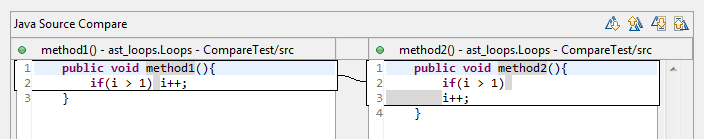
\includegraphics[scale=0.6]{Figures/introduction/intro-code-example}\\[0.1cm]
  \caption[Text to text comparison example]{The simplest example of text-to-text comparison indicating that text compare sometimes is not enough to investigate code difference, however there are no changes regards the application logic}
  \label{fig:intro-code-example}
\end{figure}

	
Since this article includes comparison not only of source code, but also Java byte code, where there is no syntax. Basically to have a look at byte code example, there are no bounds to hold a functions or methods. Based on this, control flow graph can be derived from byte code, that represents a graph, but not a spanning tree. Every node has a reference to byte code address.

%TODO: is any idea how to optimize spanning tree(node has a byte code address, topologically sort)

%TODO: find java bytecode example and his tree

%IDEA: text difference highlight and in parallel nodes in Tree marks and Matching
%(TODO: make some experiments, if it's ok, better, worse or same compare)

%EDIT:
To investigate code comparison, two algorithms of structural compare are required, in fact Top down maximum common subtree and Bottom Up maximum common subtree algorithms. To make a contribution into development of structured code compare, the following tasks should be explored:

\begin{enumerate}
  \item The existing algorithms must be investigated (The text-compare method is not sufficient to find a similarity in code)
  \item The algorithms for the structured compare(Abstract syntax trees, Control flow graphs) must be explored 
  \item New methods and algorithms find a place to tried out. A prototypes of combination text-compare and structure-compare can be implemented.
  \item Experimental results of compare must be derived.
\end{enumerate}
%EDIT

%-----------------------------------------------------
% 3nd Chapter: Graphs comparisons algorithms
%-----------------------------------------------------
\chapter{Graphs comparisons algorithms}
\label{cha:algorithms-to-compare}

This chapter is concerned with the issue of an important generalization of tree isomorphism, mostly known as Maximum Common Sub-tree isomorphism. The goal of these algorithms is finding a largest common sub-tree between two trees. It plays a major role either in scientific fields or in fundamental problems. The trees can be searched for most common sub-tree from top to down, correspondingly form the head of tree till leaves, or from bottom to up, that means the search for largest sub-tree starts from leaves upwards. The algorithms are provided by Gabriel Valiente. In his book \emph{Algorithms on Trees and Graphs} he presented detailed information about Top Down Max Common Sub-tree and Bottom Up Max Common Sub-tree isomorphism. The algorithms have been implemented in dr. Garbage tools for plugin eclipse integrated development environment. 

Further research in this area may include not only the implementation of algorithms but also their application field. On this grounds, that the algorithms can be very helpful for tree similarity investigation. The current chapter includes an explanation of how these two algorithms have implemented in the project, about auxiliary algorithms and how they can be helpful for code comparison.

\section{An algorithm for Top-down maximum common sub-tree isomorphism }
\label{sec:topdown}

There are two types of top-down maximum common sub-tree isomorphism algorithms. One of them finds the largest common ordered sub-tree $T$ between $ T_{1}$ and $ T_{2}$ such can found in both trees, by that when the sequence of edges from parent node does make a sense. On the contrary, the second type is the same top-down algorithm that takes into account the order of edges of parent node, during the algorithm execution. 

A top-down common sub-tree of two unordered trees $ T_{1}$ and $ T_{2 }$ is an unordered tree $T$ such that there are top-down unordered sub-tree isomorphisms of $ T$ into $ T_{1}$ and into $ T_{2}$. A maximal top down common sub-tree of two unordered  trees $ T_{1}$ and $ T_{2}$ is a top-down common sub-tree of $ T_{1}$ and $ T_{2}$ which is not a proper sub-tree of any other top-down common sub-tree of $ T_{1}$ and $ T_{2}$. A top-down of two unordered trees $ T_{1}$ and $ T_{2}$ is a top-down common sub-tree of $ T_{1}$ and $ T_{2}$ with the largest number of nodes \cite{valiente}.

\textbf{Definition 3.1}. \emph{
A \textbf{top-down common sub-tree} of an unordered tree $ T_{1} = ( V_{1}, E_{1})$ to another unordered tree $ T_{2} = ( V_{2}, E_{2})$ is a structure 
$ (X_{1}, X_{2}, M)$, where $ X_{1} = (W_{1}, S_{1})$ is a top down unordered subtree of $ T_{2}$ and $M \subseteq W_{1} \times  W_{2}$ is an ordered tree isomorphism of $ X_{1}$ to $ X_{2}$. A top-down common sub-tree $ (X_{1}, X_{1}, M)$ of $ T_{1}$ to $ T_{2}$ is \textbf{maximal} if there is no top-down common sub-tree of $ (X_{1}', X_{2}', M')$ of $ T_{1}$ to $ T_{2}$ such that $ X_{1}$  is a proper top-down common sub-tree of $ X_{1}'$ and $ X_{2}'$ is a proper top-down sub-tree of $ X_{2}'$, and it is \textbf{maximum} if there is no top-down common sub-tree $ (X_{1}', X_{2}', M')$  of $ T_{1}$ to $ T_{2}$ with the $size[X_{1}] < size[X_{1}']$\cite{valiente}.
}

%PICTURE TDMC
\begin{figure}[hb]
  \centering
  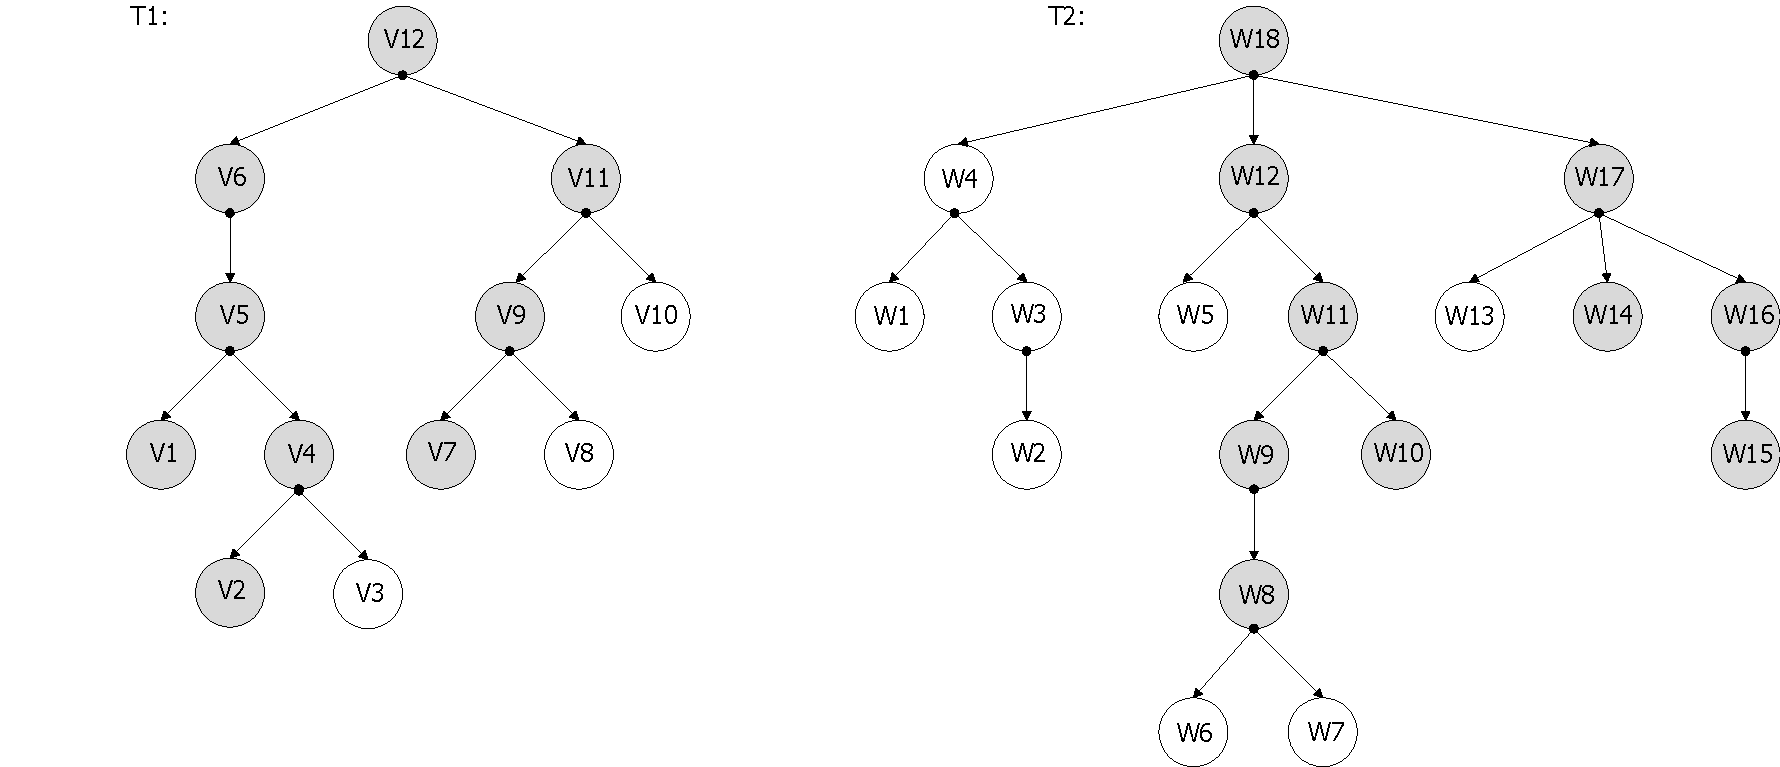
\includegraphics[scale=0.45]{Figures/algorithms/TD/top-down-max-common-example-adjusted.pdf}\\[0.1cm]
  \caption[Top-down maximum common ordered sub-tree of two unordered trees T1 and T2]{Top-down maximum common ordered sub-tree of two unordered trees T1 and T2. Nodes are numbered according to the order in which they are visiting during a post order traversal. The gray highlighted nodes are shaped maximum common sub-tree starting from the root \cite{valiente}.}
  \label{fig:top-down-max-common-example-adjusted}
\end{figure}

The figure \ref{fig:top-down-max-common-example-adjusted} demonstrates a partial injection $M \subseteq W_{1} \times  W_{2}$ among trees $ T_{1} = ( V_{1}, E_{1})$ and  $ T_{2} = ( V_{2}, E_{2})$ where $M  = \{ (v1,w10),  (v2,w8), (v4,w9), $ \\
$(v5,w11),  (v6,w12),  (v7,w15),  (v9,w16), $  $ (v10,w14),  (v11,w17),  (v12,w18)\}$ is unordered top-down maximum common sub-tree isomorphism $ T_{1}$ and $ T_{2 }$ \cite{valiente}.

Important to realize that the injection $M \subseteq W_{1} \times  W_{2}$ can contain different pairs of nodes, as a result there are is only one unique maximum common sub-tree available. Nevertheless the number of pairs of nodes is constant and always maximal.

If nodes $v$ is leaf $ T_{1}$ and $w$ is leaf of $T_{2 }$ accordingly mapped to each other, then the maximum common sub-tree gains size 1. Let suppose that $p$ is number of children of $ T_{1}$ and $q$ is number of children of $ T_{2}$ respectively. Consequently $ v_{1},...,v_{p}$ and $ w_{1},...,w_{q}$ are children of 
 $v$  and $w$\cite{valiente}. Solving the algorithm needs to build a bipartite graph $G=(\{v_{1},...,v_{p}, w_{1},...,w_{q} \}, E)$ on $p+q$ vertices, with edge 
$ v_{i},w_{i} \in E$  if and only if the size of maximum common sub-tree of the sub-tree $ T_{1}$ rooted at node $ v_{i}$ and the sub-tree of $T_{2 }$ rooted at node $ w_{i}$ is non zero\cite{valiente}. 
The bipartite graphs are built recursively the algorithm in one of trees $ T_{1}$ or $ T_{2}$ a leaf reaches. Let the leaf node of $ v_{i}$ of tree $ T_{1}$ is found, then a bipartite graph can be formed with node $ w_{i}$ from $ T_{2}$ at the same hierarchy level. Using the algorithm of \emph{Maximum Bipartite Matching} the corresponding parent nodes $ w_{i+1}$ and $ v_{i+1}$ gains weight one plus \emph{Maximum Bipartite Matching}(shortly named MBM)of current bipartite graph.

%PIC 1
\begin{figure}
  \begin{minipage}[h]{0.60\linewidth}
    \centering
    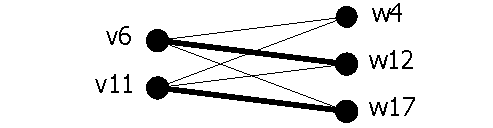
\includegraphics[scale=0.95]{Figures/algorithms/TD/1ex.pdf}\\[0.1cm]
    
  \end{minipage}%
  \begin{minipage}[b]{0.30\linewidth}
    \centering
\begin{tabular}{|c|c|c|c|}
\hline
    & w4 & w12                       & w17                       \\ \hline
v6  & 3  & \cellcolor[gray]{0.9} 5 & 3                         \\ \hline
v11 & 4  & 5                         & \cellcolor[gray]{0.9}4 \\ \hline
\end{tabular}
\end{minipage}
\caption{The solution MBM of bipartite graph brings $5+4=9$ weight from previous solutions}
\label{fig:ex1}
\end{figure}
%PIC 1

%PIC 3
\begin{figure}[h]
  \begin{minipage}[h]{0.60\linewidth}
    \centering
    
\includegraphics[scale=0.95]{Figures/algorithms/TD/3ex.pdf}\\[0.1cm]
  \end{minipage}%
  \begin{minipage}[h]{0.30\linewidth}
    \centering
\begin{tabular}{|c|c|}
\hline
   & w2 \\ \hline
v1 &  \cellcolor[gray]{0.9}1  \\ \hline
v4 & 1  \\ \hline
\end{tabular}
\end{minipage}
\caption{The $v_{1}$ and $v_{4}$ are leaf nodes of the left branch of $ T_{1}$, and leaf node $w_{2}$ of $ T_{2}$. The edge $(v_{1},v_{4})$ is selected with \emph{MBM} algorithm. }
\label{fig:ex3}
\end{figure}
%PIC 3

%PIC 2
\begin{figure}
  \begin{minipage}[h]{0.60\linewidth}
    \centering
    
\includegraphics[scale=0.95]{Figures/algorithms/TD/2ex.pdf}\\[0.1cm]
  \end{minipage}%
  \begin{minipage}[b]{0.30\linewidth}
    \centering
	\caption{The edge $(v_{5},v_{3})$ gains weight equal to two from previous solution\ref{fig:ex3}, due to the parent node}
\begin{tabular}{|c|c|c|}
\hline
   & w1 & w3                        \\ \hline
v5 & 1  & \cellcolor[gray]{0.9} 2 \\ \hline
\end{tabular}
\end{minipage}
\caption{}
\label{fig:ex2}
\end{figure}
%PIC 2

As an example can be taken from figure \ref{fig:ex1}. As said, the nodes are being traversed until leaf node in the trees $ T_{1}$ or $ T_{2}$ is found. Let consider the left branch of $ T_{1}$, namely leaves $v_{1}$ and $v_{4}$ and respectively the left branch of $ T_{2}$, namely leaf $w_{2}$. A created bipartite graph is depicted at figure  \ref{fig:ex3}. The corresponding table shows weights of edges. Since these two are leaves they equal one. With algorithms \emph{MBM} the edge $v_{1}$ and $w_{2}$ is being selected. Once the selection is done, the algorithm take their parent nodes, accordingly $v_{5}$, $w_{3}$ and $v_{3}$. The appropriate bipartite graph is constructed. The edges  $v_{5}$ and $w_{3}$ have weight equal to one initially in table \ref{fig:ex2}, but since from previous solution \ref{fig:ex3}  the node $v_{1}$ has a parent $v_{5}$, the edge $(v_{5},w_{3})$ gets weight equal to two. Likewise the edge  $(v_{6},w_{4})$ in table \ref{fig:ex1} has a value three based on previous result.

By the same way all entries in table \ref{fig:ex1} have been built. Passing through the tree $ T_{1}$ at another left branch until leaves $v_{2}$ and $w_{3}$ the similar bipartite graph can be formed \ref{fig:ex6}. As said before, the current edges get same weight equal to one. The edge $(v_{2},w_{8})$ is selected regards the \emph{MBM} algorithm. Under those circumstances the next bipartite graph can be built \ref{fig:ex5}. Based on previous solution the edge $(v_{4},w_{9})$ obtains weight equal to two.

%PIC 6
\begin{figure}[h]
  \begin{minipage}[h]{0.60\linewidth}
    \centering
    
\includegraphics[scale=0.95]{Figures/algorithms/TD/6ex.pdf}\\[0.1cm]
  \end{minipage}%
  \begin{minipage}[b]{0.30\linewidth}
    \centering
\begin{tabular}{|c|c|}
\hline
   & w8 \\ \hline
v2 & \cellcolor[gray]{0.9} 1  \\ \hline
v3 & 1  \\ \hline
\end{tabular}
\end{minipage}
\caption{Starting from leaves select of both trees select edges with maximum weight. According to the algorithm the connection $(v_{2},w_{8})$ has been selected.}
\label{fig:ex6}
\end{figure}
%PIC 6

%PIC 5
\begin{figure}[h]
  \begin{minipage}[h]{0.60\linewidth}
    \centering
    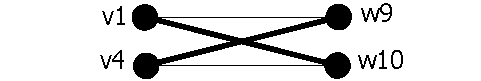
\includegraphics[scale=0.95]{Figures/algorithms/TD/5ex.pdf}\\[0.1cm]
    
  \end{minipage}%
  \begin{minipage}[b]{0.30\linewidth}
    \centering
\begin{tabular}{|c|c|c|}
\hline
   & w9 & w10 \\ \hline
v1 & 1  & \cellcolor[gray]{0.9} 1   \\ \hline
v4 &  \cellcolor[gray]{0.9}2  & 1   \\ \hline
\end{tabular}
\end{minipage}
\caption{Since previous decision was $(v_{2},w_{8})$, and they respectively are parents of $(v_{4},w_{9})$ its weight of edge gains one plus the decision equal to one.}
\label{fig:ex5}
\end{figure}
%PIC 5

%PIC 4
\begin{figure}[h]
  \begin{minipage}[h]{0.60\linewidth}
    \centering
    
\includegraphics[scale=0.95]{Figures/algorithms/TD/4ex.pdf}\\[0.1cm]
    
  \end{minipage}%
  \begin{minipage}[b]{0.30\linewidth}
    \centering
\begin{tabular}{|c|c|c|}
\hline
   & w5 & w11 \\ \hline
v5 & 1  &  \cellcolor[gray]{0.9} 4   \\ \hline
\end{tabular}
\end{minipage}
\caption{The the sum maximum matched edges from \ref{fig:ex5} equal to 3, in the same manner the edge $(v_{5},w_{11})$ gains 3 + 1 = 4 weight}
\label{fig:ex4}
\end{figure}
%PIC 4

Having a look at table in \ref{fig:ex1} in cell $(v_{6},w_{12})$ where the value is 5. This has been formed due to the solution from table \ref{fig:ex4}, because nodes $(v_{6},w_{12})$ are direct parents of $(v_{5},w_{11})$. likewise all other leaves in both trees are investigated and on-fly the tables with weight are filled out. The table in \ref{fig:ex1} is completed by the same way as described above. At the end the maximum bipartite matching algorithm selects the edges $(v_{6},w_{12})$ and $(v_{11},w_{17})$ because they bring the maximum weight of the bipartite graph. In this case two branches in \ref{fig:top-down-max-common-example-adjusted} are picked and the corresponding nodes are grey highlighted forming the maximum common sub-tree from the bottom.
Pseudo code is represented  below:

\begin{lstlisting}
list<node, node> topDownMaxCommonSubtreeIsomorphism(const TREE T1, const TREE T2){
node r1 = root(T1);
node r2 = root(T2);
traverse(node r1, node r2);
M = list<node, node>
reconstruct(r1, M);
}
\end{lstlisting}

This method goes recursively simultaneously through T1 and T2 till leaves of them are founded.
\begin{lstlisting}
void traverse(node v, node w){
int p = v.getNumberOfChildren();
int q = w.getNumberOfChildren();
if(p == 0 or q == 0) return 1;

Array matrix = new Array[p][q];

for(i = 0; i < p; i++){
	for(j = 0; j < q; j++){
		node vChild = v.getChild();	
		node wChild = w.getChild();
		matrix[i][j] = <vChild, wChild, -1>
	}
}

int res = 1;
if(p != 0 and q != 0){
bipartiteGraph bg = createBipartiteGraphFromMatrixEntry(matrix);
if (bg.numberOfEdges == 0) return 0;

list<edge> L = MaxWeightedBipartiteMatching(bg);
forall(e, L){
result += e.getCounter();
}
matching(list<edge> L);
return res;
}
}
\end{lstlisting}
This method reconstructs the top-down max common unordered sub-tree isomorphism mapping.
\begin{lstlisting}
reconstruct(node r1, list<node, node> M){
M[r1] = r2;
list<node> L;
preorder-tree-traversal(L, T1);
forall(node v, L){
	forall(node w, B[v]){
	if(M[T1.parent(v)] == T1.parent(w)){
		M[v] = w;
		break;	
	}
}
}
\end{lstlisting}
%TODO: redo this code
Puts into list B matched edges for further reconstruction
\begin{lstlisting}
matching(list<edge> L){
forall(e, L){
B[r1].insert(r2);
}
}
\end{lstlisting}

\section{An algorithm for Bottom-Up maximum common sub-tree isomorphism }
\label{sec:bottomup}

There are two types of bottom-up maximum common sub-tree isomorphism algorithms. One of them finds the largest common ordered sub-tree $T$ between $ T_{1}$ and $ T_{2}$ such can found in both trees, by that when the sequence of edges from parent node does make a sense. On the contrary, the second type is the same top-down algorithm that takes into account the order of edges of parent node, during the algorithm execution. 

A bottom-up common sub-tree of two unordered trees $ T_{1}$ and $ T_{2 }$ is an unordered tree $T$ such that there are top-down unordered sub-tree isomorphisms of $ T$ into $ T_{1}$ and into $ T_{2}$. A maximal bottom-up common sub-tree of two unordered  trees $ T_{1}$ and $ T_{2}$ is a bottom-up common sub-tree of $ T_{1}$ and $ T_{2}$ which is not a proper sub-tree of any other bottom-up common sub-tree of $ T_{1}$ and $ T_{2}$. A bottom-up of two unordered trees $ T_{1}$ and $ T_{2}$ is a bottom-up common sub-tree of $ T_{1}$ and $ T_{2}$ with the largest number of nodes \cite{valiente}.

\textbf{Definition 3.1}. \emph{
A \textbf{bottom-up common sub-tree} of an unordered tree $ T_{1} = ( V_{1}, E_{1})$ to another unordered tree $ T_{2} = ( V_{2}, E_{2})$ is a structure 
$ (X_{1}, X_{2}, M)$, where $ X_{1} = (W_{1}, S_{1})$ is a bottom-up unordered subtree of $ T_{2}$ and $M \subseteq W_{1} \times  W_{2}$ is an ordered tree isomorphism of $ X_{1}$ to $ X_{2}$. A bottom-up common sub-tree $ (X_{1}, X_{1}, M)$ of $ T_{1}$ to $ T_{2}$ is \textbf{maximal} if there is no bottom-up common sub-tree of $ (X_{1}', X_{2}', M')$ of $ T_{1}$ to $ T_{2}$ such that $ X_{1}$  is a proper bottom-up common sub-tree of $ X_{1}'$ and $ X_{2}'$ is a proper bottom-up sub-tree of $ X_{2}'$, and it is \textbf{maximum} if there is no bottom-up common sub-tree $ (X_{1}', X_{2}', M')$  of $ T_{1}$ to $ T_{2}$ with the $size[X_{1}] < size[X_{1}']$\cite{valiente}.
}

%PICTURE OF BUMC
\begin{figure}[th]
  \centering
  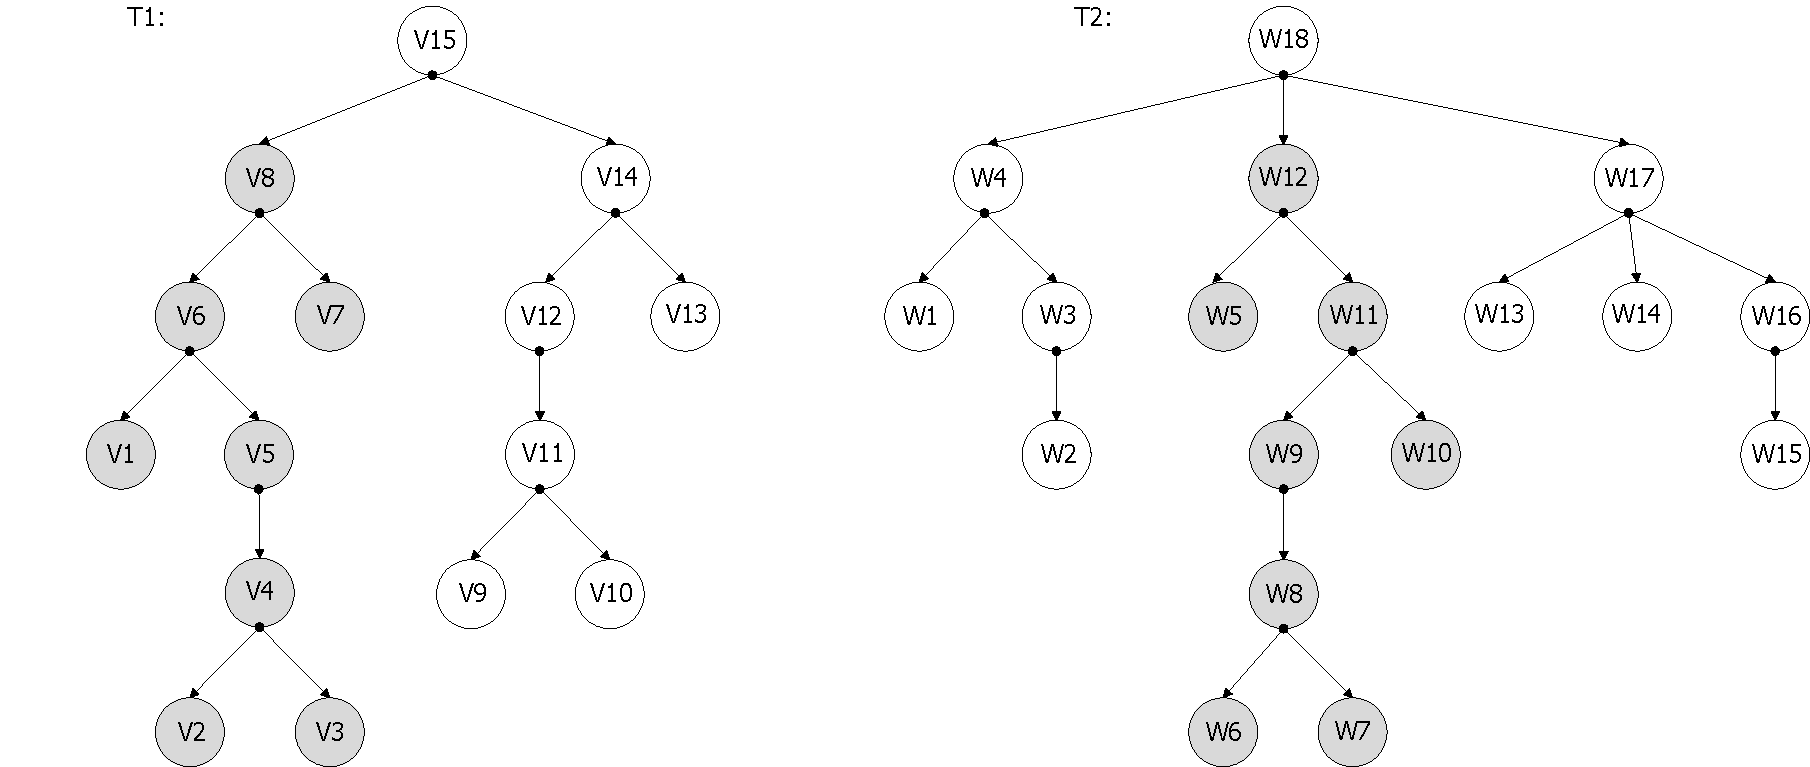
\includegraphics[scale=0.45]{Figures/algorithms/BU/bottom-up-max-common-example.pdf}\\[0.1cm]
  \caption[Bottom Up maximum common ordered sub-tree of two unordered trees T1 and T2]{Bottom Up maximum common ordered sub-tree of two unordered trees T1 and T2. Nodes are numbered according to the order in which they are visiting during a post order traversal. The gray highlighted nodes are shaped maximum common sub-tree starting from the leaves \cite{valiente}.}
  \label{fig:bottom-up-max-common-example}
\end{figure}


%-----------------------------------------------------
% 4th Chapter: Code compare experiments
%-----------------------------------------------------

\chapter{Code compare experiments}
\label{cha:experimental}
\section{Introduction to experiments}

For better understanding of possible "code compare" concept, possible ideas of implementation and following development an amount of experiments are required.
In order to build a proper tool or at least a concept, in Eclipse plugins at Dr. Garbage Community\textregistered \enspace some hand experiments in code should be fulfilled.

All these test cases are performed in Eclipse IDE \cite{eclipse_site} and divided into blocks. These steps can be approached by following:

\begin{enumerate}
  \item Research on Java source code using existing methods to compare:
  	\begin{enumerate}
   	 	\item Normal text compare
   		 \item Spanning trees transformed from control flow graphs
	 \end{enumerate}	
	 
  \item Research on Java source code using existing methods to compare:
  \begin{enumerate}
    \item Normal text compare 
    \item Abstract syntax trees
  \end{enumerate}
  
  \item Research on Java byte code using existing methods to compare:
  \begin{enumerate}
    \item Normal text compare 
    \item Control flow graphs
  \end{enumerate}
\end{enumerate}

All test set are investigated under Java methods and functions. Playing around with the patterns of code changing variables, names, sequences of commands, adding loops or conditions and apply the simple "text to text" compare. This "text compare" is already implemented in Eclipse IDE \cite{eclipse_site}, so-called command "compare with each other by member". This type of comparison provides a pop-up window, where two pieces of code are compared, line by line.

TODO: Add Text compare picture

In parallel a control flow graphs or source graphs from the functions are being created and compared using implemented algorithms Top-Down and Bottom-Up(following called: TD\& BU). The further task is to figure out the difference/similarity from graphical visual comparison. Consequently these both results must be matched and recorded for succeeding research.

The derived results from can be as follows: 
\begin{enumerate}
  \item Text compare and TD \& BU have same difference
  \item Text compare and TD \& BU give similar difference
  \item Text compare and TD \& BU five full difference
\end{enumerate}

Hence, as it was declared in section description of problem, based on these results can be decided what kind of tool in Dr. Garbage Eclipse plug-ins can be built.In case similar or full difference results, a combination of both methods can be used for optimal comparison. 

Small example can be demonstrated: there are two functions that look very similar but nevertheless they have different number of string and different functionality. The abstract results can be following:
\begin{enumerate}
	\item Text compare shows that strings 1 and 5 are different
	\item Graph compare shows that string 7 is different 
\end{enumerate}

Conclusion: a combination of two methods can explicit that strings 1,5 and 7 are distinguished and much more distinction has been found. Thus it provides an optimal way of investigation.


% TEXT COMPARE HOW IT WORKS

TODO: explain briefly how TEXT compare works(search in internet ), and sometimes it's not enough to observe the difference

% JAVA SOURCE CODE EXPERIMENTS

\section{Experiments on Java source code Flowcharts}

A flowchart is a type of diagram that represents an algorithm, workflow or process, showing the steps as boxes of various kinds, and their order by connecting them with arrows. This diagrammatic representation illustrates a solution model to a given problem. Flowcharts are used in analyzing, designing, documenting or managing a process or program in various fields\cite{wiki_flowchart}.

Dr. Garbage tools\cite{drgarbage} provides a solution how to represent sequential flowchart alongside to Java source code(see figure \ref{fig:java-flowchart-example}).
\begin{figure}[h]
  \centering
  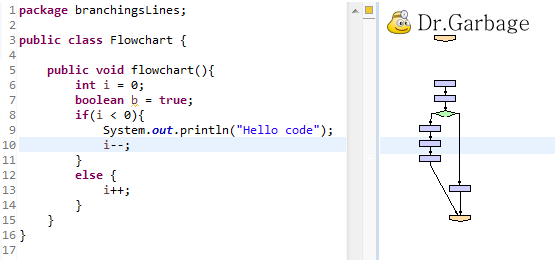
\includegraphics[width=1.00\textwidth]{Figures/Java-flowchart-exp/java-flowchart-example.png}\\[0.1cm]
  \caption[Java sequential block diagram opened in Java Source code Visualizer]{Example of source code visualizer}
  \label{fig:java-flowchart-example}
\end{figure}

A depicted flowchart can be easily extracted into control flow graph (see figure \ref{fig:control-flow-graph}). If there is another similar function, it can be transformed into next control flow graph. These two graphs are being compared using existing TDMC[\ref{sec:topdown}] and BUMC[\ref{sec:bottomup}] algorithms. 

\begin{figure}
  \centering
  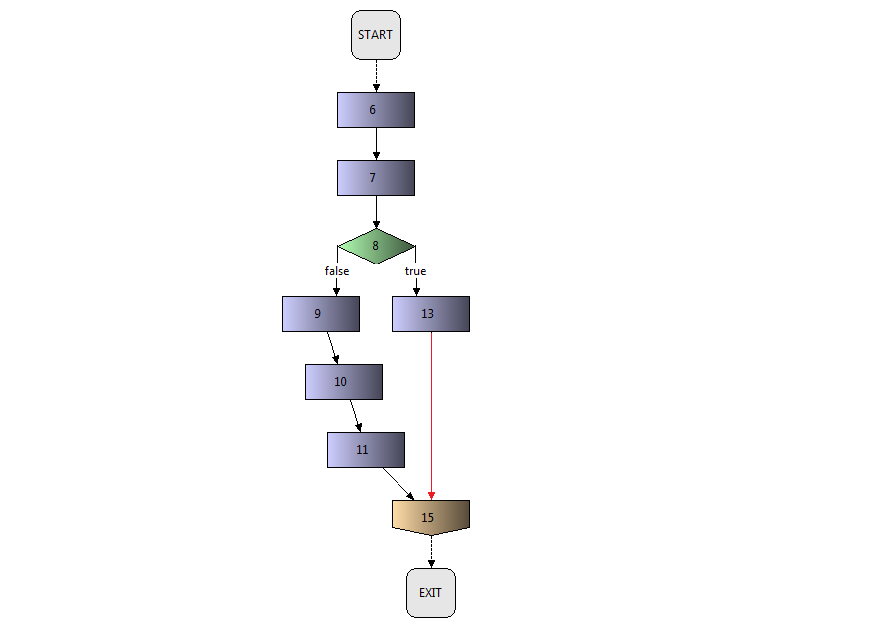
\includegraphics[width=1.00\textwidth]{Figures/Java-flowchart-exp/control-flow-graph.png}\\[0.1cm]
  \caption[Extracted control flow graph from Java source code]{Extracted control flow graph from Java source code}
  \label{fig:control-flow-graph}
\end{figure}

Unfortunately these two algorithms are applicable only for tree structures. For this reason this problem can be reduced, removing minimum number of edges to get a spanning tree. Thus the the edges in the input graphs are reduced by Spanning Tree Algorithm[\ref{sec:graph-transformation}]. The removed edges are red highlighted, hence this for this structure TDMC and BUMC[\ref{cha:algorithms-to-compare}] can be easily applied.

To conduct an experiments a sequence of actions and following statistic are needed. After conducted experiments, taking into account the derived statistic, a conclusion takes place. The steps are carried through sequence of action:
\begin{itemize}
	\item Write two similar functions in Eclipse IDE
	\item Apply for them text-to-text comparison
	\item Declare the statistic, respectively how many lines are different		
	\item Create a source-code graph for both
	\item Apply TD \& BU algorithms to get structural difference	
	\item Declare the statistic, respectively how many nodes are different			
\end{itemize}

In this section all experiments have been executed by hand using plug-in tool "Graph Comparison" in Eclipse from dr. Garbage project. Before starting, a several rules how to evaluate code difference in text and in graph must be established. It is one of the crucial moment, because followed data statistic are used in further tool development.

For the estimation of structural difference there are criteria listed:
\begin{itemize}
	\item Each java operator is considered as simple node
	\item Changing a conditions of block on the contrary issues 100\% difference of business logic, however the structure stays unchangeable.
	\item Availability of extra variables in second piece of code is calculated by division of number of extra variables to amount of all variables.
\end{itemize}

Mostly all calculations are performed by roughly, because there are many criteria how to evaluate the logic and structure difference. But from this perspective these rules are enough to examine graph's similarity.

For the text difference found via Eclipse tool a criteria to evaluate can be added:
\begin{itemize}
	\item Percentage is computed by number of 
	\item If in one line of code only one symbol has been covered as found, then it is division of one to amount of symbols in this line. 
\end{itemize}

\begin{figure}
  \centering
  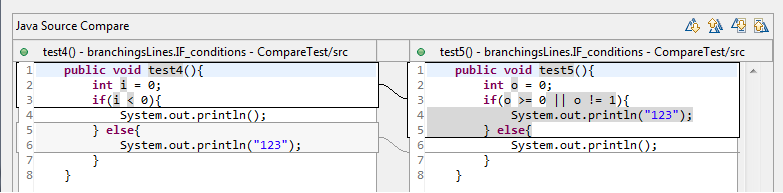
\includegraphics[width=1.00\textwidth]{Figures/Java-flowchart-exp/example-graph.png}\\[0.1cm]
  \caption[Two pieces of code are being compared with Eclipse Text Comparison]{Two pieces of code are being compared with Eclipse Text Comparison}
  \label{fig:example-graph}
\end{figure}

And after generation of two graphs, these both are compared(see the figure \ref{fig:graphs-compared}) using existing TDMC and BUMC[\ref{cha:algorithms-to-compare}] algorithms.
\begin{figure}
  \centering
  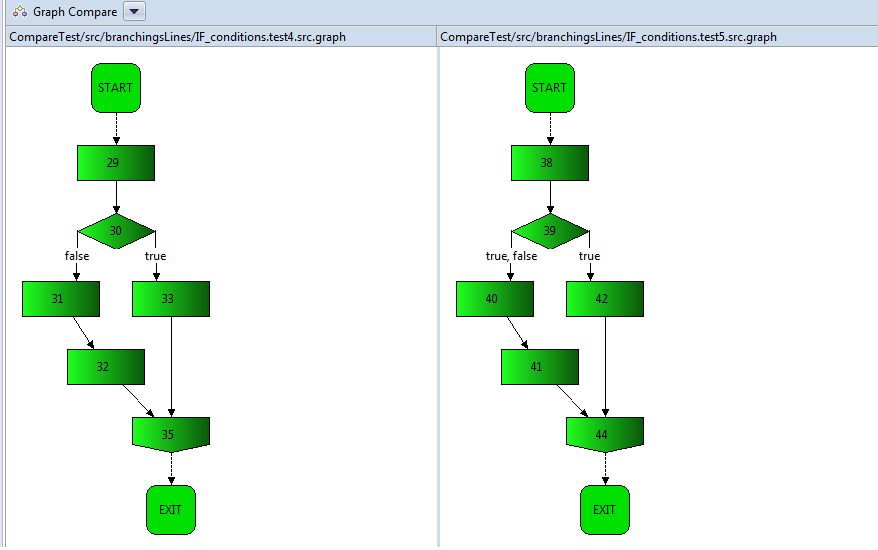
\includegraphics[width=1.00\textwidth]{Figures/Java-flowchart-exp/graphs-compared.png}\\[0.1cm]
  \caption[Compared source code graphs using TDMC algorithm \ref{sec:topdown} ]{Compared source code graphs using TDMC algorithm}
  \label{fig:graphs-compared}
\end{figure}


\begin{table}[h]
\begin{tabular}{|c|c|c|c|c|}
\hline
\multicolumn{3}{|c|}{Compare experiments}                & Text -to-text compared     & Graphcompared              \\ \hline
Test id & Name of functions & \begin{tabular}[c]{@{}c@{}}Real  code \\ difference \%\end{tabular} & \begin{tabular}[c]{@{}c@{}}Layout difference\\  \% found\end{tabular} & TD\&BU similarity \% found \\ \hline
1       & t1() and t2() &             50             &             100               &               100             \\ \hline
2       & t1() and t3() &               50           &                   100         &            75                \\ \hline
3       & t1() and t4() &                50          &             100               &              100              \\ \hline
4       & t1() and t2() &                50          &        100                    &                80            \\ \hline
5       & t1() and t5() &                50          &            100                &            100                \\ \hline
6       & t6() and t7() &               33           &                33            &               100             \\ \hline
7       & ti1() and ti2() &              10            &                100            &             0               \\ \hline
8       & ti2() and ti3() &             16             &                100            &              100              \\ \hline
9       & ti3() and ti4() &               25           &         100                   &                 66           \\ \hline
10      & ti4() and ti5() &                 50         &           100                 &                   0         \\ \hline
11      & ti6() and ti7() &                 90         &           100                 &                   42         \\ \hline
\end{tabular}
\caption{The table demonstrates results of Java Source comparison using text-to-text compare method and application of algorithms to their source code graphs }
\label{table:tests-table}
\end{table}

The table \ref{table:tests-table} shows results of java source code experiments. Existing algorithms [\ref{cha:algorithms-to-compare}] and Eclipse text-to-text comparison have been used to reveal the best approach of code comparison. As it said above, the difference code can be figured out either structurally or simple text comparison. Based on the table \ref{table:tests-table} the apparent conclusion are composed:

\begin{itemize}
	\item If the application logic is totally different (For example \textbf{if conditions}) then Eclipse Text Compare finds the difference, thus condition itself is highlighted. The graphical comparison with TD\& BU are not able to see this distinction. It is obvious since graph theory in this case is able to find 
how similar structure of code fragments. The conducted example \ref{fig:graphs-compared} above can testify this conclusion. In this way graph theory is not applicable to differentiate logic of application.
	
	\item In opposite said above, the graphical compare is quite useful instrument to investigate a code structure. For example, if another third party person has changed local variables, the structure remains same, thus TDMC\& BUMC (especially TDMC) find high level of similarity. Unfortunately this approach is not enough to build a new concept allowing to investigate the difference more precisely.
	
	\item The graph is totally bound to lines of codes. If one brace is shifted, then it's considered one more block in the graph(Dr. Garbage Source Code Visualizer \cite{drgarbage} generates extra node for each code operator). Hence TDMC is not able to find following branch where there an extra node and generated Java source code graph is not optimized for comparison.
	
	\item Text-to-text compare is enough to investigate a text difference because this tool finds every different sub-string in code line. But as stated above, changing variables, sequence of operators or even production same loops with different operators the text-to-text compare find too much unmatched strings. Eventually the result of text compare looks like a disorder with same and unmatched sub-strings.  	
	

\end{itemize}

% JAVA AST TREE CODE EXPERIMENTS
\section{Experiments using Abstract Syntax Tree graphs}

In this section the abstract syntax trees are generated from Java source code using Dr. Garbage plugins \cite{drgarbage}.
The most notable advantage of building AST trees is a direct converting Java source code into AST tree, thereby avoiding graphs with cycles. Thus there is no need to delete back edges(see Spanning tree algorithms).

TODO: short explanation about AST how it looks like;

In this section all experiments have been executed by hand using plug-in tool "Graph Comparison" in Eclipse from dr. Garbage project \cite{drgarbage}.  Before starting, a several rules how to evaluate code difference in text and in graph must be established. It one of the crucial moment, because followed data statistic are used in further tool development.


TODO: after this compares write a conclusion what is better to compare

IDEA: compare AST
AST optimization, for each node the label must be equal to the corresponding value in the code.
go through the nodes, and compare the values in the nodes.
Optimization: substitute some AST construction like \texttt{i++;} to the \texttt{i = i + 1;}, helps to find similarity
AST native trees will more abstract (almost the same as JAVA compiler converts any code to ).
ATTACH tree AST and AST native

ARTICLE:
Parsing: In case of parse tree-based approaches, the entire source code base is parsed to build parse tree or (annotated) abstract syntax tree (AST). In such representation, the source unit and comparison units are represented as subtrees of the parse tree or AST. Comparison algorithm then uses these subtrees to find clones [31, 213, 222]. Metrics-based approaches may also use such representation of code to calculate of the subtrees and find clones based on the metrics values [146, 178].

\begin{lstlisting}
public void test1(){
		int frameGroupLine = 10;
		for(int Cnt = 1; Cnt < frameGroupLine;  Cnt =+ 2)
		{
			if(Cnt*4 != 2){
				frameGroupLine++;
			}
		}
	}
	
public void test2(){
		int frameGroupLine = 10;
		for(int Counter = 1; Counter < frameGroupLine;  Counter =+ 2)
		{
			if(Counter*4 != 2){ 
				frameGroupLine = frameGroupLine + 1;
			}
		}
	}	
\end{lstlisting}

If this line \texttt{frameGroupLine = frameGroupLine + 1;} will be converted into one format of sub-tree, that indicates the same as \texttt{frameGroupLine++;}. Thus this sub-tree can be found with TDMC or BUMC algorithms. Consequently it brings more covered nodes that signalize more similarity. 

\begin{lstlisting}
	public void test3(){
		int frameTeamLine = 10;
		for(int i = 1; i < frameTeamLine;  i =+ 2)
		{
			if(i*4 != 2){ 
				frameTeamLine++;
			}
		}
	}
\end{lstlisting}

The code fragments test1() and test2() have the same application logic but different variables. However in the second one the increment of variable "frameTeamLine" is differently written. From text to text compare the functions are different at this point. If the text code similarity will be calculated, then these two fragments are not same(probably 90\% similarity). Using Abstract Syntax Trees Optimization, this types of structure can be converted in the same sub-tree of whole AST tree. Thereby these two different text structures are represented as same sub-tree. 

\vspace{4mm}

\begin{figure}[h]
  \centering
  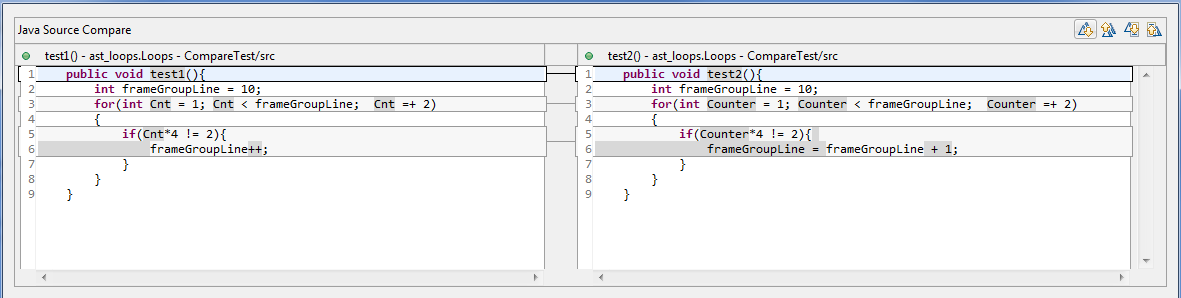
\includegraphics[width=1.00\textwidth]{Figures/AST-optimization/text-to-text-compare}\\[0.1cm]
  \caption[Text to text comparison example]{Example of standard text-to-text comparison of Java code}
  \label{fig:text-to-text-compare}
\end{figure}

On figure \ref{fig:text-to-text-compare} the example demonstrated how these two functions are compared using Eclipse Text comparison window. After creation and comparison these two AST trees, it can be easily seen that sub-trees (the increment) are different.

\begin{figure}[h]
  \centering
  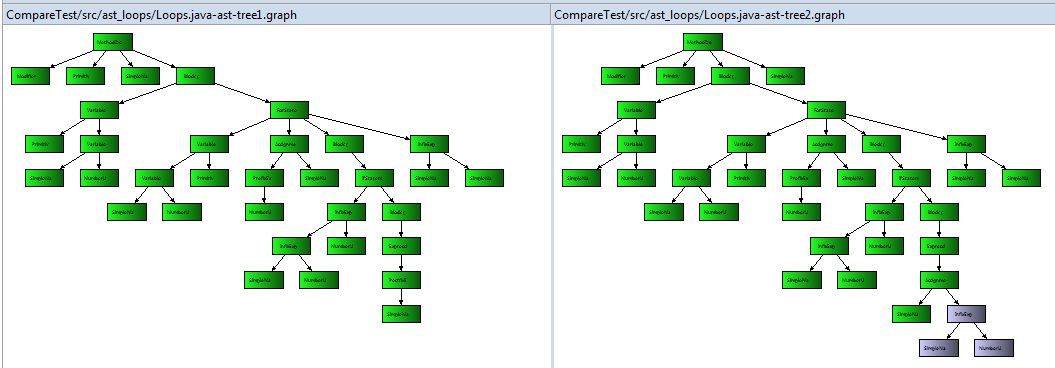
\includegraphics[width=1.00\textwidth]{Figures/AST-optimization/tree-compared1}\\[0.1cm]
  \caption[Graph comparison on similar AST trees]{Graph comparison of function test1() and test2() using TDMC algorithm \ref{sec:topdown}}
  \label{fig:ast-graph-compare-similar-tdmc}
\end{figure}

From the figure \ref{fig:ast-graph-compare-similar-tdmc} TDMC algorithm finds incomplete code similarity since not all nodes have been covered. From statistical point of view using simple math, the percentage of similarity is figured out: 37 nodes in the test2() and 3 of them are not covered. Thus, the calculation indicates  $\left ( 1 - \left (\frac{3}{37} \right ) \right )\cdot 100 = 91\%$ code similarity according to AST trees and applied TDMC algorithm.

This mismatch can be optimized during AST tree production. These two lines of code \texttt{frameGroupLine++;} and \texttt{frameGroupLine = frameGroupLine + 1;}
must be built as a same sub-tree, accordingly same structure and same number of nodes. Using this simple replacement it allows to built a similar AST trees, when logic is same but the source code text is different. Consequently the converted AST trees to some extent are independent from source code and can be compared to explicit the difference.

% JAVA AST TREE CODE EXPERIMENTS
\section{Experiments on JavaByte Code}
\label{sec: java-code-experiments}

In this section an investigation regards java byte-code comparison is expound. Unlike Java source code, the corresponding byte code has practically no application logic. In spite of this the topic must be researched for the clone detection.

\begin{figure}[ht]
  \centering
  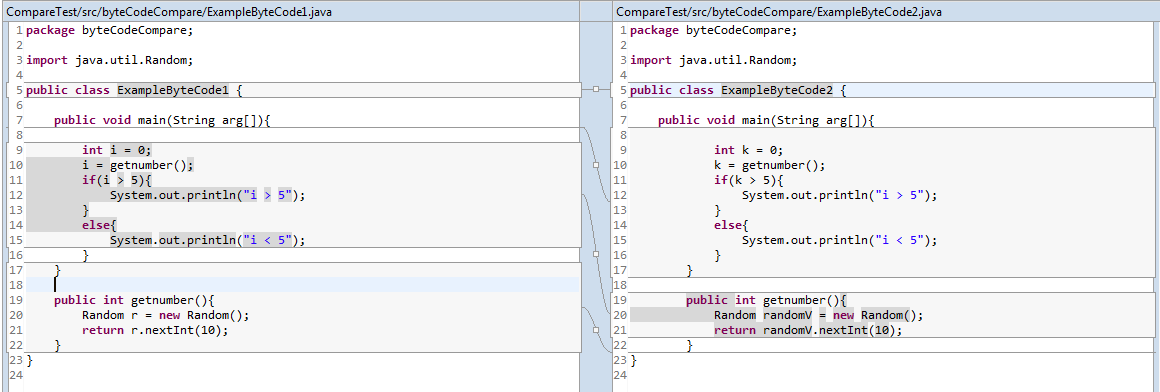
\includegraphics[width=1.00\textwidth]{Figures/bytecode-compare/example-of-bytecode-original-compared}\\[0.1cm]
  \caption[Functions compared by members]{Java source code compared using text-to-text}
  \label{fig:example-of-bytecode-original-compared}
\end{figure}


\begin{figure}[h]
  \centering
  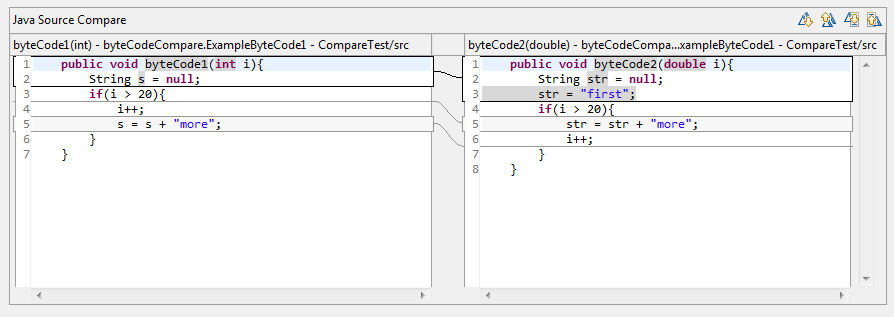
\includegraphics[scale = 0.55]{Figures/bytecode-compare/example-of-bytecode-text-compared}\\[0.1cm]
  \caption[Functions compared by members]{Java byte code compared using text-to-text}
  \label{fig:example-of-bytecode-text-compared}
\end{figure}

%-----------------------------------------------------
% 5th Chapter: Graph transformation algorithms
%-----------------------------------------------------


\chapter{Graph transformation algorithms}
\label{cha:graph-transformation}

\section{Introduction to the graph transformation}
\label{sec:graph-transformation}

TODO: explain how graph is generated, which libraries are used, plugins

\section{Techniques to build a tree from code}
TODO: what is AST, examples;
\\
TODO: what is BasicBlock, examples;

\section{Convert graph to tree}
\label{sec: generate-to-tree}
TODO: decribe here how to remove edges in order to get spanning tree

\section{Possible ideas}


%-----------------------------------------------------
% 6th Chapter: Graph transformation algorithms
%-----------------------------------------------------
\chapter{Existing Comparison methods}
\section{Plagiarism detection methods}

Task of plagiarism detection is an identification of text's similarity. Thus a research of existing methods is useful for this work regards code's comparison.
\begin{quote} Plagiarism detection is the process of locating instances of plagiarism within a work or document. The widespread use of computers and the advent of the Internet has made it easier to plagiarize the work of others. Most cases of plagiarism are found in academia, where documents are typically essays or reports. However, plagiarism can be found in virtually any field, including scientific papers, art designs, and source code \cite{wiki_plagiarism}. \end{quote}

Mostly the task of plagiarism detection is considered for many fields, like text documents, software and source code. In this chapter source code plagiarism is being reviewed.

According to the article of Chanchal Kumar Roy and James R. Cordy \cite{software_clone_detection}, source-code similarity detection 
algorithms can be classified :
\begin{itemize}
	\item Text-based Techniques
	\item Token-based Techniques
	\item Tree-based Techniques
	\item PDG-based Techniques
	\item Tree-based Techniques
	\item Metrics-based Techniques
\end{itemize}



%-----------------------------------------------------
% 5th Chapter: Conclusion
%-----------------------------------------------------

\chapter{Conclusion}
\label{cha:Conclusion}

TEMP
based on experimental results and own opinion, write here what results were derived 
From time to time write here combined conclusions or improvements



%-----------------------------------------------------
% Literature
%-----------------------------------------------------

\newpage
%\bibliographystyle{plain}
\begin{thebibliography}{100} % 100 is a random guess of the total number of references 
\addcontentsline{toc}{chapter}{Bibliography}
%Example:
%\bibitem{ch11} George H.L. Fletcher and Catharine M. Wyss, "Data Mapping as Search", Computer Science Department, School of Informatics, Indiana University, Bloomington, USA. 

 \bibitem{drgarbage}The Dr. Garbage Tools Project\textregistered \enspace 2014, Sergej Alekseev, Peter Palaga and Sebastian Reschke, URL:
\url{http://www.drgarbage.com}

 \bibitem{graph_compare} Sergej Alekseev. \emph{ Graph theoretical algorithms for control flow graph comparison}, 2013.
 
\bibitem{valiente} Gabriel Valiente,\emph{Algorithms on Trees and Graphs}, Berlin: Springer-Verlag, 2002.

\bibitem{wiki_flowchart} Free content Internet encyclopedia - Wikipedia: Flowcharts, URL: \url{https://en.wikipedia.org/wiki/Flowchart}

\bibitem{wiki_plagiarism} Free content Internet encyclopedia - Wikipedia: Plagiarism detection, URL: \url{http://en.wikipedia.org/wiki/Plagiarism_detection}
 
\bibitem{software_clone_detection} Roy, Chanchal Kumar; Cordy, James R. (September 26, 2007). \emph{"A Survey on Software Clone Detection Research".} School of Computing, Queen's University, Canada.

\bibitem{graph_isomorphism_is} Koebler Johannes; Schoening, Uwe. (July 29, 1991). \emph{"GRAPH ISOMORPHISM IS LOW FOR PP".} Theoretische Informatik, Universitaet Ulm


\bibitem{eclipse_site} Eclipse documentation, URL: \url{http://help.eclipse.org/luna/index.jsp}



\bibitem{sample1} Sample Author, NAME,
(Berlin: Springer-Verlag, 2002).

\end{thebibliography} 

\end{document}
